\section{Semantic rules}

\subsection{EPNs}

 \begin{enumerate}
   \item All \glyph{state variables} associated with a Stateful Entity Pool Node should be unique and not duplicated within that node.
   \item If a state variable is used in one EPN then is must be used in all equivalent stateful EPNs\footnote{A stateful EPN is equivalent if the EPNs are identical when their state descriptions are ignore.}.
   \item EPNs should not be orphaned (i.e.\, they must be associated with at least one arc.
%    \item A \glyph{complex} should consists of different EPNs. If two or more 
%    elements of the complex are identical they should be replaced by multimer. 
 \end{enumerate}

\subsection{Process Nodes}

As described in \sect{process}, the \glyph{consumption} and \glyph{production} arcs converge before connecting to the process node (\fig{process-sidedness}). This defines the EPNs that are the input and outputs of an irreversible process. Since, processes can be reversible in the following rules we refer to these groupings as the ``left-hand-side'' (LHS) and ``right-hand-side'' (RHS) of the process\footnote{Note this designation is purely for grouping and is used even then the sides of the reaction are above and below the process.}. For convenience we will also collectively refer to the \glyph{consumption} and \glyph{production} arcs as \emph{flux} arcs.

\begin{figure}[H]
  \centering
  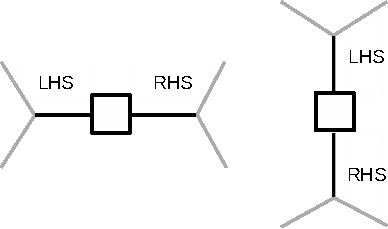
\includegraphics[scale = 0.4]{images/process_sidedness}
  \caption{An illustration of the ``sidedness'' of a process. The designation of LHS and RHS is essentially arbitrary.}
  \label{fig:process-sidedness}
\end{figure}

\subsubsection{Flux Arcs}

\begin{enumerate}
\item All process nodes (with the exception of \glyph{phenotype}) must have a LHS and RHS.
    \item All EPNs on the LHS of a process must be unique.
    \item All EPNs on the RHS of a process must be unique.
    \item All \glyph{phenotype} glyphs must be associated with at least one modulation arc.
    \item The EPNs that make up the LHS of the process should be consistent with the RHS, i.e.\, the process should constitute a    balanced biochemical reaction.
    \item Once the stoichiometry of a flux arc is displayed in a map then all other flux arcs should
    display theit stoichiometry make.
    \item If the stoichiometry is undefined or unknown this should be indicated by the use of a question mark (``?''). 
   \item If more than one set of stoichiometries can be applied to the flux arcs of the process then the stoichiometry of the flux arcs must be displayed.
%     \item \glyph{PNs} should have only one \glyph{Catalysis} arc connected to them. If
%     there more than one catalyst known to affect the process, several \glyph{PNs} should be
%     drawn or a \glyph{logical operator} used 
%     \item \glyph{PNs} should have only one \glyph{necessary stimulation} arc connected to it. If
%     there is more than one \glyph{EPN} acting as a necessary stimulator on a process, then a \glyph{logic operator} should be used.
\end{enumerate}  

\subsubsection{\glyph{Association}}

  \begin{enumerate}
    \item An \glyph{Association} is always an irreversible process.
\end{enumerate}  

\subsubsection{\glyph{Dissociation}}
  \begin{enumerate}
    \item An \glyph{Dissociation} is always an irreversible process.
\end{enumerate}  

\subsubsection{Modulation}
\label{sec:mod-semantics}

As discussed in \sect{concepts}, it is implied, but not defined explicitly that the process has a rate at
which it converts its LHS EPNs to its RHS EPNs (and vice-versa in the case of a reversible process). This concept is
important in understanding how the \PDl describes process modulation.

\begin{enumerate}
\item A \glyph{process} with no modulations has an underlying ``basal rate''
  which describes the rate at which it converts inputs to outputs.
\item A \glyph{modulation} changes the basal rate in an unspecified fashion.
\item A \glyph{stimulation} is a modulation that increases the basal rate.
\item An \glyph{inhibition} is a modulation that decreases the basal rate.
\item The above types of modulation, when assigned to the same process, are combined and have a multiplicative effect on the basal rate of the process.
\item Modulators that do not interact with each other in the above manner, should be drawn as modulating different process nodes. Their effect is therefore additive.
\item At most one \glyph{necessary stimulation} can be assigned to a process node. Two \glyph{necessary stimulations}
  would imply an implicit AND or OR operator. For clarity only
  one \glyph{necessary stimulation} can be assigned to a \glyph{process}, and such combinations must be
  explicitly expressed using \glyph{logical operators}.  \item At most one \glyph{catalysis} can be assigned to a \glyph{process}. A catalysis arcs
  modulation implies that the exact biochemical mechanism underlying
  the process is known. In this context two \glyph{catalysis} cannot
  be assigned to the same process node as they represent
  independent reactions. Other EPNs can be
  assigned to the same process than a catalysis, such as modulators, stimulators, and
  inhibitors, and will have a multiplicative modulation on the reaction
  rate defined by the catalysis.
\end{enumerate}

\subsubsection{Reversible Processes}
\label{sec: semantics reversible procs}

A process is deemed to be reversible if it has \glyph{production} arcs on both the LHS and RHS of a process node \fig{process-reversibility}. Semantically, the \glyph{production} arc can be thought of as allowing a reversible flow of entities between the \glyph{process} and the \glyph{EPN}. A \glyph{consumption} arc only permits an irreversible flow from the \glyph{EPN} to the \glyph{process}. In this way, the \glyph{consumption} arc forces the \glyph{process} to be irreversible. \glyph{Consumption} arcs cannot be associated with both sides of a \glyph{process} as this would prohibit any flow through the \glyph{process}.

\begin{figure}[H]
  \centering
  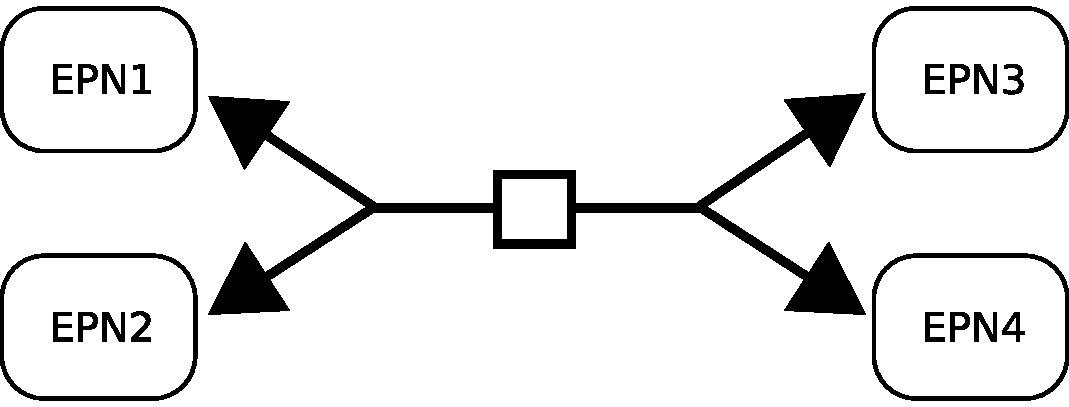
\includegraphics[scale = 0.4]{images/reversible_process}
  \caption{A valid reversible process. A process is reversible if its LHS and RHS contain only \glyph{production} arcs.}
  \label{fig:process-reversibility}
\end{figure}
 
\begin{enumerate}
\item  A mixture of \glyph{consumption} and \glyph{production} arcs on the same side of a \glyph{process} is not permitted.
\item A \glyph{sink} cannot be linked to a reversible process as it only receives entities, and so would effectively make the process irreversible\footnote{A \glyph{source} can only be associated with a \glyph{consumption} arc so this rule does not apply in this case.}.
\item The semantics of \glyph{modulation} is the same as for irreversible processes, .i.e. the amount of entity in the modulation pool affects the rate of the process.
\end{enumerate}

 
\subsection{Cloning}

SBGN allows identical nodes to be duplicated on a map if they are
explicitly marked as such. This is done using a \glyph{clone marker}. The details are shown in table \ref{tab:processduprules}.


\begin{center}
\tablecaption{Duplication rules.}
\label{tab:processduprules}
\begin{footnotesize}
\tablefirsthead{\hline
  Node & Can be duplicated & Indication & Additional Rules\\\hline}
\tablehead{\hline
\multicolumn{4}{|l|}{\small\sl continued from previous page}\\
\hline\hline
  Node & Duplicate? & Indication & Additional Rules\\\hline\hline}
\tabletail{\hline
\multicolumn{4}{|r|}{\small\sl continued on next page}\\
\hline}
\tablelasttail{\hline}
\begin{supertabular}{|l|c|p{4cm}|p{3.5cm}|}\hline
%  Node & Duplicate? & How & Additional Rules\\\hline
Compartment   & N & & \\\hline
SimpleChemical & Y & \glyph{Simple clone marker} & \\\hline
UnspecifiedEntity & Y & \glyph{Simple clone marker} & \\\hline
Source & N & & \\\hline
Sink & N & & \\\hline
Perturbing Agent & Y & \glyph{Simple clone marker} & \\\hline
Phenotype & Y & \glyph{Simple clone marker} & \\\hline
MultimerChemicalEntity & Y & \glyph{Simple clone marker} & \\\hline
StatefulEntityPool & Y & \glyph{Labeled clone marker} & \\\hline
Macromolecule & Y & \glyph{Labeled clone marker} & \\\hline
MultimerMacromolecule & Y & \glyph{Labeled clone marker} & \\\hline
Nucleic\-Acid\-Feature & Y & \glyph{Labeled clone marker} & \\\hline
Complex & Y & \glyph{Labeled clone marker} & \\\hline
Process & Y & None & Duplication is implied when all EPNs linked to the Process are marked as clones.\\\hline
OmittedProcess & Y & As Process  & \\\hline
UncertainProcess & Y & As Process  & \\\hline
Association & Y & As Process  & \\\hline
Dissociation & Y & As Process  & \\\hline
LogicalOperator & Y & None & \\\hline
AND & Y & None & \\\hline
OR & Y & None & \\\hline
NOT & Y & None & \\\hline
\end{supertabular}
\end{footnotesize}
\end{center}


\subsection{Compartment spanning}

An \glyph{EPN} cannot \emph{belong} to more than one
\glyph{compartment}. However, an EPN can be \emph{drawn} over more than one
\glyph{compartment}. In such cases, the decision on which is the owning
\glyph{compartment} is deferred to the drawing tool or the
author. A \glyph{complex} may contain EPNs which belong to different
\glyph{compartments} and in this way a \glyph{complex} can be used to describe
entities that span more than one {compartment}.

This restriction makes it impossible to represent in a semantically
correct way a macromolecule that spans more then one compartment ---
for example a receptor protein. It is clearly desirable to be able to
show a macromolecule in a manner that the biologist expects (i.e.\,
spanning from the outside through the membrane to the
inside). Therefore, the author is recommended to draw the
macromolecule across compartment boundaries, but the underlying SBGN
semantic model will assign it to only one. The assignment to a
\glyph{compartment} may be decided by the software drawing tool or the
author. Note that this has implications for auto-layout algorithms as
they will only be able to treat such \glyph{entity pool nodes} as contained within
a \glyph{compartment} and will have no way of knowing a macromolecule spans a
compartment.

The current solution is consistent with other Systems Biology
representations such as SBML and BioPAX. For more information about the
problems representing membrane spanning proteins and the rationale
behind the current solution see \sect{postponed}.

\subsection{Submaps}

The submap is a visual device that allows the detail of an \PD map to be exported into another \PD map and replaced by a \glyph{submap} glyph, which acts as a place-holder. This is described and illustrated in \sect{submap}. In the following discussion we will refer to the original map as the \emph{main} map and the map containing the export detail as the submap. 

\begin{enumerate}
\item For a valid mapping between an EPN in the map and submap to exist the identifiers in the \glyph{tag} and the submap terminal must be identical and their associated entity pool nodes must be identical.
\item If the same EPN is present in the map and a submap, then they must be mapped to each other.
\item Since the main map and submap share the same namespace, an EPN that is cloned in the main map must also be
marked as cloned in the submap --- even if there is only one copy of the EPN in the submap. The converse applies when the EPN in the submap is cloned\footnote{This has the additional benefit of ensuring that main maps and submaps do not need to be modified if the submap is exanded and collapsed by a viewing or editing tool.}.
\end{enumerate}

% \section{Summary of Rules}

% This section summarises the rules of SBGN-PD in a form that is intended to be accessible to tool developers and those interested in validating process maps. Each rule has been given an identifier for ease of reference. Note that no meaning is attached to the rule identifier and any perceived ordering of the identifiers is not significant.

% \subsection{Entity Pool Nodes}

% \begin{description}
% \item[PD1] The identity of an EPN is defined by a combination of its compartment, entity type (e.g. complex or macromolecule), name and state variables (if any).
% \item[PD2] A Complex’s identity consists of the identity of its subunits and a name is optional. All complexes with the same name should have the same subunits.
% \item[PD3] An EPN may belong to only one compartment.
% \item[PD4] An EPN belongs to only one compartment. If no compartment is draw it is assumed to belong to a “default” compartment.
% \item[PD5] An EPN can overlap more than one compartment and in this case it is deferred to the drawing tool or author to assign the owning compartment. Note this rule need not apply in cases where SBGN is draw by hand.
% \item[PD6] A Complex may contain subunits that belong to different compartments (the complex itself will belong to only one, however).
% \item[PD7] The layout or organisation of a compartment does not imply anything about its topology.
% \item[PD8] The layout or organisation of the EPNs in a complex does not imply any information about topology.
% \item[PD10] Complexes can be nested. This does imply information about the complex’s topology.
% \item[PD11] A complex should consist of different EPNs. If two or more elements of the complex are identical then they should be replaced by a multimer.
% \item[PD12] Source and sink nodes must have no name and be attached to only one consumption or production arc.
% \item[PD13] An EPN must be connected to at least 1 consumption, production or modulation arc.
% \item[PD14] An EPN is not allowed to be a substrate and product of the same process. This applies to cloned EPNs as well.
% States
% \item[PD15] All state variables in a stateful EPN should have different names.
% \item[PD16] A blank state variable has the value “unset”.
% \item[PD17] The state of a complex is the sum of its subunits’ and its own state variables.
% \item[PD48] The \glyph{Sink} cannot be linked to a reversible process.
% \end{description}

% \subsection{Compartments}

% \begin{description}
% \item[PD18] Compartments cannot be nested. Compartments may overlap, but overlap does not imply containment.
% \item[PD19] The layout or organisation of a compartment does not imply anything about its topology.
% \item[PD20] If no compartment is draw it is assumed to belong to a “default” compartment.
% \item[PD21] If one or more compartment glyphs are drawn then all EPNs must owned by a compartment glyph.
% \end{description}

% \subsection{Process Nodes (PN)}

% \begin{description}
% \item[PD22] A Process Node should have non-zero number of consumption and production links.
% \item[PD23] All substrates of the Process Node should be different. If several copies of the same EPN are involved in the process, the cardinality label of consumption arc should be used.
% \item[PD24] All products of the PN should be different. If several copies of the same EPN are produced in the process, the cardinality label of production arc should be used.
% \item[PD25] Once the cardinality label is added to one arc connected to a PN all other such arcs should display a cardinality label.
% \item[PD26] The cardinality of an arc can be undefined or unknown, in which case a question mark (``?'') should be used.
% \item[PD27] A PN should correspond to only one process or series of connected process. The same set of EPNs should be connected by different PNs if they are consumed and produced by different processes.
% \item[PD28] The composition of the products of an association process should be equivalent to its substrates
% \item[PD29] The composition of the products of a dissociation process should be equivalent to its substrate.
% \end{description}

% \subsection{Modulation and Logical Operators}

% \begin{description}
% \item[PD30] A PN with no modulations has an underlying “basal rate” which describes the rate at which it converts inputs to outputs.
% \item[PD31] Modulation changes the basal rate in an unspecified fashion.
% \item[PD32] Stimulation is a modulation that’s effect is to increase the basal rate.
% \item[PD33] Inhibition is a modulation that’s effect is to decrease the basal rate.
% \item[PD34] The above types of modulation, when assigned to the same process are combined and have a multiplicative effect on the basal rate of the process.
% \item[PD35] Modulators that do not interact with each other in the above manner should be drawn as modulating different process nodes. Their effect is therefore additive.
% \item[PD36] At most one trigger can be assigned to a process. Two triggers would imply an implicit Boolean AND or OR operator, so for clarity only one trigger can be assigned to a process and such combinations must be explicitly expressed as the Boolean operators.
% \item[PD37] The PN should have only one Catalysis arc connected to it. A catalysis modulation implies that the exact biochemical mechanism underlying the process is known.
% \item[PD38] The PN should have only one Trigger arc connected to it.
% \item[PD39] AND and OR Boolean logic gates should have two or more input and one output.
% \item[PD40] A NOT gate can only have one input and output.
% \end{description}

% \subsection{Cloning and Sub-Maps}

% \begin{description}
% \item[PD41] Duplicate EPNs must be marked as clones.
% \item[PD42] Duplicate stateful EPNs must use a Labelled Clone Marker.
% \item[PD43] Duplicate non-stateful EPNs must use a simple clone marker.
% \item[PD44] A sub-map shares the same namespace as its main map.
% \item[PD45] To map an EPN in the main map to one in a sub-map, the SubMap glyph in the main map must contain an identifier that matches the identifier of a Tag in the sub-map. Both EPNs must be identical.
% \item[PD46] If a main map and a sub-map contain an identical EPN then a mapping must exist between them.
% \item[PD47] If an EPN is cloned in the main map, then it must be marked as cloned in the sub-map, with the same identifier in both maps. This is true if there is only one EPN of this type in the submap.
% \end{description}
